\documentclass[12pt,a4paper]{article}
\usepackage[fontset=windows]{ctex} % 使用ctex包来支持中文
\usepackage{xeCJK}
\usepackage{fontspec}
\usepackage{graphicx}
\usepackage{fancyhdr}
\usepackage{geometry}
\usepackage{ragged2e}
\usepackage{xcolor}
\usepackage{adjustbox} % 用于调整图像位置和大小
\usepackage{subcaption}
% 设置中文字体
\setCJKmainfont{SimSun} % 宋体
\setCJKsansfont{SimHei} % 黑体
\setCJKmonofont{FangSong} % 仿宋
\newCJKfontfamily\kaiti{KaiTi} % 楷体
% 设置英文字体
\setmainfont{Times New Roman} % 使用Times New Roman
% 设置页面边距
\DeclareGraphicsExtensions{.pdf, .jpg, .tif, .png}
\thispagestyle{empty}
\vspace*{-16ex}

% 设置页面边距
\geometry{left=2.5cm, right=2.5cm, top=3cm, bottom=3cm}
% 设置全局左对齐
\setlength{\parindent}{2em} % 设置段落缩进
\begin{document}
\centerline{
\begin{tabular}{*3{c}}
    \parbox[t]{0.4\linewidth}{
    \begin{center}\includegraphics[width=\linewidth]{"left.png"}
    \end{center}}
    & \parbox[t]{0.3\linewidth}{
    \begin{center}
    \CJKfontspec{KaiTi} % 使用黑体
    \Huge% 设置字体大小为Huge
    \textbf{\Huge 天然药物化学实验报告}
    \end{center}}
    & \parbox[t]{0.4\linewidth}{
     \begin{center}
\includegraphics[width=\linewidth]{right.jpg}\end{center}} \\
    \hline
\end{tabular}
}
%\begin{center}
%
\includegraphics[width=\linewidth]{logo.jpg}
%\end{center}
\centering

\includegraphics[width=0.8\linewidth]{logo.jpg}\\[24pt] % Change the 
 % 左对齐
%\raggedright
 %   {\Huge\textbf{实验名称:}} {\LARGE 闪击波兰}\\[28pt]
 %   {\Huge\textbf{学生姓名:}} {\LARGE 拿破仑 $\cdot$ 波拿巴}\\[28pt]
%    {\Huge\textbf{学号:}} {\LARGE 114514}\\[28pt]
%    {\Huge\textbf{指导教师:}} {\LARGE 汤姆 $\cdot$ 哈克}\\[28pt]
%    {\Huge\textbf{组别:}} {\LARGE 带英}\qquad{\Huge\textbf{同组成员:}} %{\LARGE 汉弗莱 $\cdot$ 阿普比}\\[28pt]
 %   {\Huge\textbf{实验日期:}} {\LARGE 1812年莫斯科的那一场雪}\\
 %\justifying % 恢复默认对齐
     \raggedright
    {\Huge\textbf{实验名称:}} {\LARGE 霍格沃茨魔药课实验}\\[28pt]
    {\Huge\textbf{学生姓名:}} {\LARGE 哈利 $\cdot$ 波特}\\[28pt]
    {\Huge\textbf{学号:}} {\LARGE 394627}\\[28pt]
    {\Huge\textbf{指导教师:}} {\LARGE 赛弗勒斯 $\cdot$ 斯内普}\\[28pt]
    {\Huge\textbf{组别:}} {\LARGE 格兰芬多}\qquad{\Huge\textbf{同组成员:}} {\LARGE 赫敏 $\cdot$ 格兰杰}\\[28pt]
    {\Huge\textbf{实验日期:}} {\LARGE 1996年6月1日}\\
\vspace*{\fill}
\newpage
\pagestyle{fancy}
\fancyhf{}
\rfoot{\thepage}
%%%%%%%%%%%%%%%%%%%%%%%%%%%%%%
%目录
\newpage
\tableofcontents
\newpage
\section{实验目的}
\textbf{1.学习脂溶性生物碱和水溶性生物碱提取、分离的基本原理和方法}\\
\textbf{2.熟悉生物碱的鉴定方法}\\
\textbf{3.掌握薄层色谱、柱色谱及纸色谱的一般操作方法}\\
\section{实验原理}
无限可能
\section{实验步骤}
敬请期待
\section{实验结果与分析}
无限可能
\section{思考题}
敬请期待
\section{致谢}
\begin{figure}[h]
\centering
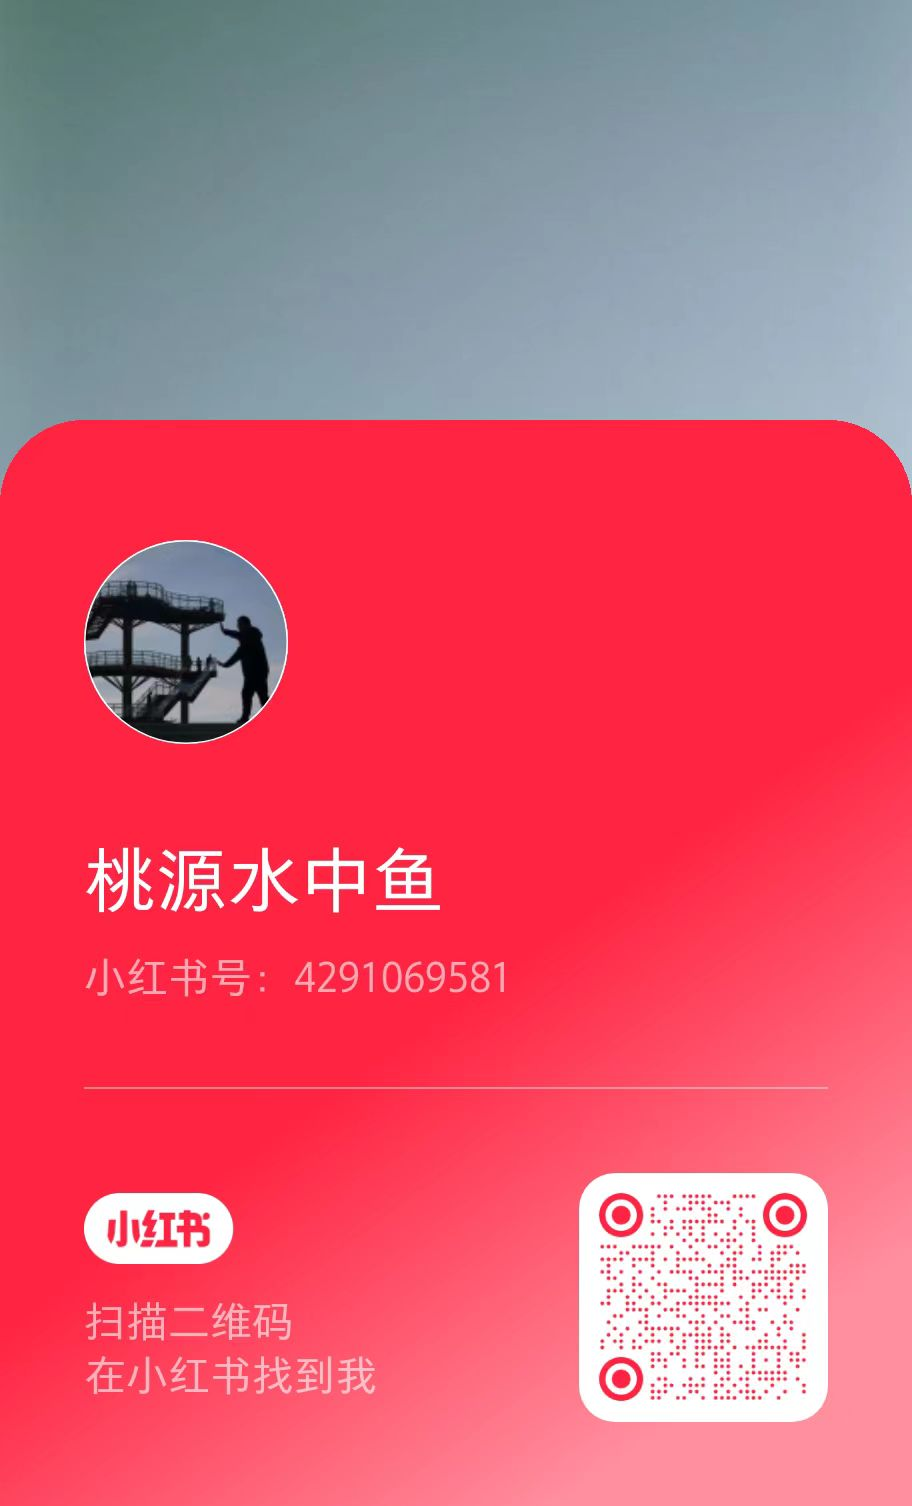
\includegraphics[width=0.2\linewidth]{red.jpg}\\[24pt]
关注我,不迷路!
\end{figure}
\end{document}
